\chapter[One-sample, two-sample and paired $t$-tests]{One-sample, two-sample\\ and paired $t$-tests}
\section{One-sample $t$-test for the mean of a normal population}
\subsection{The following are the systolic blood pressures (mm Hg) of $n = 9$ patients undergoing drug therapy for hypertension:}

\begin{center}
182.00  152.00  178.00  157.00  194.00  163.00  144.00  114.00  174.00
\end{center}


\textbf{The mean = 162 mm Hg, the standard deviation SD = 23.92.}


\begin{enumerate}[a)]
\item Find the standard error.	\hrulefill
\item Find the 95\% confidence interval for the population mean.	
	 \hrulefill

	What is the meaning of this interval? 	  \hrulefill	

\item \textbf{We would like to test whether the sample is drawn from a population where $\mu = 130$.}

Find the null- and alternative hypothesis.
	
	H$_0$:	\hrulefill
	
	H$_A$:	\hrulefill
	
	\begin{description} %[i)]
	\item[Based on the confidence interval]
	Can we conclude with 95\% confidence on the basis of these data that the population mean is different from 130? 
	Explain your decision. 
	
	\hrulefill
	
	\item[Based on the $t$ test-statistics]
	


	Is the population mean significantly different from 130 at 5\% level?
	
	$t = \frac{\textrm{mean} - 130}{SE} =$ 	\hrulefill
	
Compare its absolute value to the t-value of the table. 	 \hrulefill
		
		Explain your decision. 	\hrulefill
	\item[Based on the $p$-value]
	The $p$-value given by R is $p = 0.004$.
	
	Is there a significant difference from the hypothesized population mean 130 at 5\% level?

		\hrulefill

	\end{description}
\item \textbf{We would like to test whether the sample is drawn from a population where $\mu = 150$.}
	
Find the null- and alternative hypothesis.
		
		H$_0$:	\hrulefill
		
		H$_A$:	\hrulefill
		
		\begin{description}
		\item[Based on the confidence interval]
	Can we conclude with 95\% confidence on the basis of these data that the population mean is different from 150? 
	Explain your decision. 
	
	\hrulefill
	
	\item[Based on the $t$ test-statistics]
	


	Is the population mean significantly different from 150 at 5\% level?
	
	$t = \frac{\textrm{mean} - 150}{SE} =$ 	\hrulefill
	
Compare its absolute value to the t-value of the table. 	 \hrulefill
		
		Explain your decision. 	\hrulefill
	\item[Based on the $p$-value]
			The $p$-value given by R is $p = 0.171$.
	
			Is there a significant difference from the hypothesized population mean 150 at 5\% level?
		
				\hrulefill	
		\end{description}
\end{enumerate}
	
\section{Paired $t$-test}
\subsection{The effect of saline on the blood PH was examined in a certain disease. The blood PH value was measured two times: before the treatment and 20 minutes later, after infusion of saline ($n = 18$). Is there a significant change in mean blood PH at 5\% level? }

	\begin{minipage}{0.2\textwidth}
	\flushright
		\begin{tabular}{cc}
		\toprule
		0’&20’\\
		\midrule
		7.43&7.43\\
		7.39&7.39\\
		7.37&7.38\\
		7.43&7.42\\
		7.39&7.39\\
		7.36&7.41\\
		7.38&7.38\\
		7.39&7.39\\
		7.34&7.41\\
		7.32&7.35\\
		7.40&7.39\\
		7.32&7.33\\
		7.42&7.39\\
		7.42&7.4\\
		7.37&7.36\\
		7.37&7.39\\
		7.39&7.37\\
		7.43&7.48\\
		\bottomrule
		\end{tabular}
	\end{minipage}
	\begin{minipage}{0.7\textwidth}
		\centering
		\begin{tabular}{cccc}
		\toprule
		& \multicolumn{3}{c}{\textbf{Descriptive statistics}}	\\
		
				& 0’		& 20’ 		& difference\\
			\midrule
		mean 	& 7.3844	& 7.3922	& -0.00778\\
		SD		& 0.03485	& 0.03264	& 0.02691\\
		\bottomrule
		\end{tabular}\bigskip		
		
		mean-SD diagram: 
		
		\vspace{12em}
	\end{minipage}	
		
\begin{enumerate}[a)]
\item The name of the appropriate test: \hrulefill
\item H$_0$:	 \hrulefill


	 H$_A$:	 \hrulefill
\item $t =$ 	 \hrulefill\quad  df = \hrulefill \quad critical $t$-value ($t_\alpha$)= \hrulefill
\item Decision: 	 \hrulefill

	Conclusion: \hrulefill


\item Check your calculation using results of R.


\lstinputlisting[float=h,frame=tblr]{Code/05-ttest1.txt}


	\begin{enumerate}[i)]
	\item Find the 95\% confidence interval for the difference. 	 \hrulefill
	
	
		Decision based on the confidence interval: 		\hrulefill
	\item $t =$ 	 \hrulefill\quad df = 	\hrulefill	
	
		 Decision based on $t$-value: 	\hrulefill
	\item $p$-value = \hrulefill 
	
		Decision based on $p$-value: 	\hrulefill
	\end{enumerate}
\end{enumerate}


\subsection{The effect of Na-lactate on the blood PH was examined in a certain disease. The blood PH value was measured two times: before the treatment and 20 minutes later, after infusion of Na-lactate (n = 20). Is there a significant change in mean blood PH at 5\% level?}

	\begin{minipage}{0.2\textwidth}
	\flushright\small
		\begin{tabular}{cc}
		\toprule
		0’&20’\\
		\midrule
			7.42&7.46\\
			7.36&7.43\\
			7.4 &7.46\\
			7.43&7.48\\
			7.38&7.42\\
			7.32&7.45\\
			7.37&7.46\\
			7.36&7.48\\
			7.34&7.45\\
			7.31&7.37\\
			7.34&7.47\\
			7.37&7.43\\
			7.42&7.48\\
			7.42&7.43\\
			7.46&7.51\\
			7.37&7.41\\
			7.45&7.48\\
			7.42&7.44\\
			7.42&7.37\\
			7.41&7.45\\
		\bottomrule
		\end{tabular}
	\end{minipage}
	\begin{minipage}{0.7\textwidth}
		\centering
		\begin{tabular}{cccc}
		\toprule
		& \multicolumn{3}{c}{\textbf{Descriptive statistics}}	\\
		
				& 0’		& 20’ 		& difference\\
			\midrule
		mean 	& 7.3885	& 7.4465	& -0.058\\
		SD		& 	0.04258	& 	0.03573	& 0.04336\\
		\bottomrule
		\end{tabular}\bigskip		
		
		mean-SD diagram:
		
		\vspace{12em}
	\end{minipage}	
		
				
\begin{enumerate}[a)]
\item The name of the appropriate test: \hrulefill
\item H$_0$:	 \hrulefill


	 H$_A$:	 \hrulefill
\item $t =$ 	 \hrulefill\quad  df = \hrulefill \quad critical $t$-value ($t_\alpha$)= \hrulefill
\item Decision: 	 \hrulefill

	 Conclusion: \hrulefill


\item Check your calculation using results of R.


\lstinputlisting[float=h,frame=tblr]{Code/05-ttest2.txt}


	\begin{enumerate}[i)]
	\item Find the 95\% confidence interval for the difference. 	 \hrulefill
	
	
		Decision based on the confidence interval: 		\hrulefill
	\item $t =$ 	 \hrulefill\quad df = 	\hrulefill	
	
		 Decision based on $t$-value: 	\hrulefill
	\item $p$-value = \hrulefill 
	
		Decision based on $p$-value: 	\hrulefill
	\end{enumerate}
\end{enumerate}



	
	
\subsection{The systolic blood pressure of 6 patients was measured before and after a new drug. The mean of the sample differences is 6 mmHg, the standard error of the differences is 4.65. Is there a significant change in blood pressure at 5\% and at 1\% level?}

	\begin{minipage}{0.45\textwidth}
	$\alpha=5\%$
	
		\begin{enumerate}[a)]
		\item Appropriate test: \hrulefill
		\item H$_0:$	 \hrulefill

			 H$_A$:	 \hrulefill
		\item t: 	 \hrulefill

			degrees of freedom: \hrulefill 

			critical value: \hrulefill
		\item Decision: 	 \hrulefill

				Conclusion: \hrulefill
		\end{enumerate}
	\end{minipage}
	\hfill
	\begin{minipage}{0.45\textwidth}
		$\alpha=1\%$
		
		\begin{enumerate}[a)]
		\item Appropriate test: \hrulefill
		\item H$_0:$	 \hrulefill

			 H$_A$:	 \hrulefill
		\item t: 	 \hrulefill

			degrees of freedom: \hrulefill 

			critical value: \hrulefill
		\item Decision: 	 \hrulefill

				Conclusion: \hrulefill
		\end{enumerate}
	\end{minipage}

\subsection{The body mass of 16 patients was measured before and after a special diet. The mean of the sample differences is 5 kg, the standard deviation of the differences is 2.5. Is there a significant change in body mass at 5\% and at 1\% level?}
	
	\begin{minipage}{0.45\textwidth}
	$\alpha=5\%$
	
		\begin{enumerate}[a)]
		\item Appropriate test: \hrulefill
		\item H$_0:$	 \hrulefill

			 H$_A$:	 \hrulefill
		\item t: 	 \hrulefill

			degrees of freedom: \hrulefill  \quad 
			critical value: \hrulefill
		\item Decision: 	 \hrulefill

				Conclusion: \hrulefill
		\end{enumerate}
	\end{minipage}
	\hfill
	\begin{minipage}{0.45\textwidth}
	$\alpha=1\%$
		
		\begin{enumerate}[a)]
		\item Appropriate test: \hrulefill
		\item H$_0:$	 \hrulefill

			 H$_A$:	 \hrulefill
		\item t: 	 \hrulefill

			degrees of freedom: \hrulefill  \quad 
			critical value: \hrulefill

		\item Decision: 	 \hrulefill

				Conclusion: \hrulefill
		\end{enumerate}
	\end{minipage}


\section{Calculations with R}

\subsection{Open the file \data{befafter.csv}. A study was conducted to determine weight loss, body composition, etc. in obese women before and after 12 weeks of treatment with a very-low-calorie diet. Column \variable{BEFORE} and \variable{AFTER} contain weights of 9 women. We wish to know if these data provide sufficient evidence to allow us to conclude that the treatment is effective in causing weight reduction in obese women. Let $\alpha= 0.05$}

		
\begin{enumerate}[a)]
\item The name of the appropriate test:	 \hrulefill
\item H$_0$:	 \hrulefill\\
		 H$_A$:	 \hrulefill



		\begin{center}\small
		\begin{tabular}{lC{2cm}C{2cm}}
			\toprule	
				\textit{Descriptive statistics}		& mean & SD\\
			\midrule
			Before diet &&\\
			After diet &&\\
			difference &&\\
			\bottomrule
		\end{tabular}\medskip
	\end{center}
\item 95\% CI for the difference:  \hrulefill
	%
	\quad		Decision: 	\hrulefill
\item $t =$ 	 \hrulefill\quad degrees of freedom = 	 \hrulefill\quad $t_\alpha$=	\hrulefill	
	%
	\quad	 Decision: 	\hrulefill
\item $p$-value = \hrulefill 
	\quad	Decision: \hrulefill

\end{enumerate}


\section{Two-sample $t$-test}
\subsection{The height of secondary school girls was compared in two Hungarian cities. Decide whether the two samples are drawn from populations having the same mean (at 5\% level). Read the results from the SPSS output below.}

	\begin{center}
	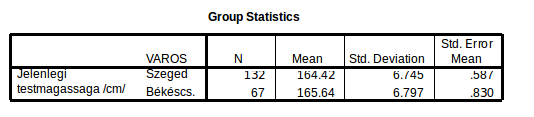
\includegraphics[width=0.6\textwidth]{SPSS/Ketmintas1}
	\end{center}

	\begin{enumerate}[a)]
	\item The name of the appropriate test:	\hrulefill
	\item H$_0$:	\hrulefill

		 H$_A$:	\hrulefill
	\item Assumptions:	\hrulefill
	\end{enumerate}
	
\subsubsection*{Equality of variances $\alpha=5\%$}
		\begin{enumerate}[a)]
%TODO
%		\item A varianciák összehasonlításához mit használ fel a fenti eredmények közül? 	\hrulefill	
		\item Check visually the equality of variances:	\hrulefill

			
		\item $F =$\hrulefill \quad df: \hrulefill \quad $F_{\textrm{table}, 0.05} = 1.64$ 
			
					p-value: \hrulefill
		\item Decision about the equality of variances: \hrulefill
		\end{enumerate}
		
\subsubsection*{Equality of population means $\alpha=5\%$}
		\begin{enumerate}[a)]
%		\item Az átlagok összehasonlításához mit használ fel a fenti eredmények közül?		\hrulefill
%		\item Mit gondol ezek alapján („szemre”) a testmagasság-átlagokról? 		\hrulefill

		\item Which $t$-test formula is appropriate here?
			\begin{enumerate}[i)]
				\item equal variances, $t$
				\item different variances, $d$
			\end{enumerate}
			
			\begin{eqnarray*}
			s_p &=& \frac{(n-1) \cdot s_x^2 + (m-1) \cdot s_y^2} { n+m-2 } = \frac{131 \cdot 6.745^2+66 \cdot 6.792^2} { 132-67-2 } = 45.73\\
			t   &=& \frac{ \bar x- \bar y }{ s_p } \cdot \sqrt { \frac{nm}{n+m} } = 
					\frac{ 164.42-165.64 }{\sqrt{45.73}} \cdot \sqrt { \frac{132 \cdot 67}{132+67 }}=-1.203
			\end{eqnarray*}
		
				\item df: \hrulefill\quad		$t$-value :	\hrulefill \quad $p$-value: 0.229 %\hrulefill
		\item Decision about the equality of population means 	\hrulefill
		
			Based on $t$-value: \hrulefill
			
			Based on $p$-value:  \hrulefill
		
		%	Van-e szignifikáns különbség a két populáció átlaga között 5\%-os szinten?	\hrulefill
		\end{enumerate}

		\textbf{Find the relevant statistical values in the SPSS output!}
		
			\begin{center}
			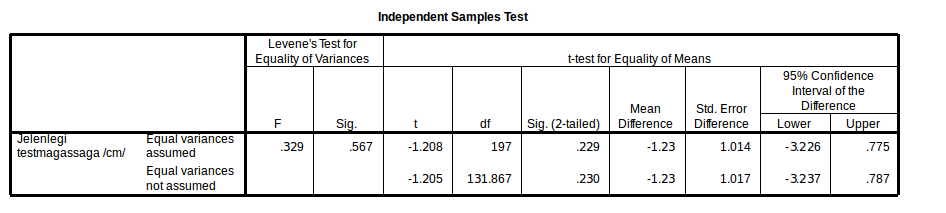
\includegraphics[width=0.9\textwidth]{SPSS/Ketmintas1b}
			\end{center}
			
\subsection{The body mass of secondary school girls was compared in two Hungarian cities. Decide whether the two samples are drawn from populations having the same mean (at 5\% level). Read the results from the SPSS output below.}

	\begin{center}
	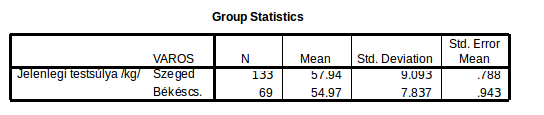
\includegraphics[width=0.7\textwidth]{SPSS/Ketmintas2a}
	\end{center}
	
	
	\begin{enumerate}[a)]
	\item The name of the appropriate test:	\hrulefill
	\item H$_0$:	\hrulefill

	H$_A$:	\hrulefill
	\item Assumptions:	\hrulefill
	\end{enumerate}
	
\subsubsection*{Equality of variances $\alpha=5\%$}
		\begin{enumerate}[a)]
		%TODO
		%\item A varianciák összehasonlításához mit használ fel a fenti eredmények közül? 	\hrulefill	
		\item Check visually the equality of variances:	\hrulefill

			
		\item $F =$\hrulefill \quad df: \hrulefill \quad $F_{\textrm{table}, 0.05} = 1,64$ 
			
					p-value: \hrulefill
		\item Decision about the equality of variances: \hrulefill
		\end{enumerate}
	
\subsubsection*{Equality of population means $\alpha=5\%$}
%		\item Az átlagok összehasonlításához mit használ fel a fenti eredmények közül?		\hrulefill
%		\item Mit gondol ezek alapján („szemre”) a testmagasság-átlagokról? 		\hrulefill


		Decision about the equality of population means 

			\begin{enumerate}[a)]
			\item 	Based on $t$-value: \hrulefill
			\item 	Based on $p$-value:  \hrulefill
		
		%	Van-e szignifikáns különbség a két populáció átlaga között 5\%-os szinten?	\hrulefill
			\end{enumerate}
		
		\textbf{Find the relevant statistical values in the SPSS output!}
		
			\begin{center}
			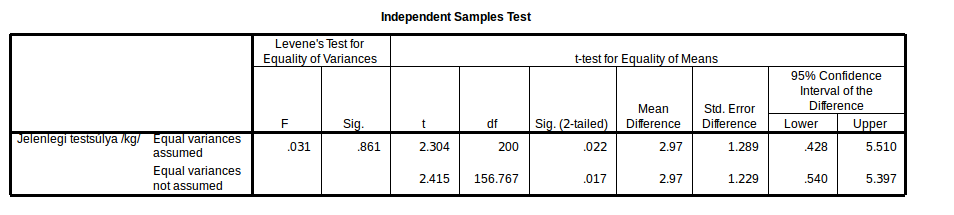
\includegraphics[width=0.9\textwidth]{SPSS/Ketmintas2b}
			\end{center}


\clearpage

\section{Calculations with R}
\subsection{Open the file \quest!\\ Compare the mean body mass of boys and girls (at 5\% level).}
	
	\begin{enumerate}[a)]
	\item The name of the appropriate test:\hrulefill
	\item H$_0$:	\hrulefill
	
		H$_A$:	\hrulefill
		
	\item Assumptions: 	\hrulefill
	\end{enumerate}
	
	
	\begin{center}
		\begin{tabular}{r|C{2cm}|C{2cm}}
		\toprule
					& boys & girls\\
		\midrule
		sample size	&&\\
		mean		&&\\
		standard deviation		&&\\
		SE			&&\\
		\bottomrule
		\end{tabular}
	\end{center}

\subsubsection*{Equality of variances $\alpha=5\%$}
		\begin{enumerate}[a)]
		\item $p$-value: \hrulefill	
		\item Decision about the equality of variances:	\hrulefill
		\end{enumerate}
		
\subsubsection*{Equality of population means $\alpha=5\%$}
		\begin{enumerate}[a)]
		\item $t=$ \hrulefill \quad df?	\hrulefill\quad			$p=$ \hrulefill
		\item 95\% CI of the difference: \hrulefill
		\item Decision about the equality of population means: \hrulefill
		\item Conclusion: \hrulefill		
		\end{enumerate}


\section{Homework}
\subsection[LWTBWT.csv]{Open the file \data{LWTBWT.csv}} 
Variable \variable{BWT} contains the body weight of the newborn babies and variable \variable{SMOKE} contains values according to the mother smoking (0 not, 1 yes). Compare the mean body weight of the babies by smoking habits of the mother. 

\subsection[ANTHROPOMETRICS.csv]{Open the file \data{ANTHROPOMETRICS.csv}}
Compare the body height of boys and girls. Find other variables to be compared and find the appropriate test.

\subsection[CALC.csv]{Open the file \data{CALC.csv}}
Here, systolic blood pressures are given before and after a calcium treatment in two groups. Find problems where paired $t$-tests can be used. Find problems where two-sample $t$-tests can be used. 

\subsection[NEWDRUG.csv]{Open the file \data{NEWDRUG.csv}}
Find problems where paired $t$-tests can be used. Find problems where two-sample $t$-tests can be used.
